\documentclass{beamer}
% --------------- PACCHETTI ---------------
% Immagini
\usepackage{graphicx} 
% Layout multicolonna
\usepackage{multicol}
% Listings
\usepackage{listings}    
% ------------- FINE PACCHETTI ---------------

\usetheme{Copenhagen}

% --------------- INTESTAZIONE ---------------
\title{Verifica funzionale di programmi con Dafny}
\author{Lorenzo Quellerba}
\institute{Università degli Studi di Torino}
\date{13 Giugno 2023}
% --------------- FINE INTESTAZIONE ---------------

\begin{document}
\maketitle
\begin{frame}{Dafny}
    \only<1>{
        \begin{columns}[onlytextwidth]
            \column{0.7\textwidth}
                \begin{itemize}
                    \item Dafny è un linguaggio di programmazione che supporta nativamente la verifica funzionale
                    \item Durante lo sviluppo, un programma Dafny viene annotato con la specifica formale del comportamento atteso
                    e automaticamente un verificatore statico (un dimostratore automatico) controlla che il codice la rispetti (\textit{correct by construction})
                    \item Il linguaggio supporta sia il paradigma imperativo che quello funzionale, i generici,
                    l'ereditarietà, l'incapsulamento, l'allocazione dinamica della memoria e i tipi di dato induttivi
                \end{itemize}
            \column{0.25\textwidth}
            \begin{figure}
                
\includegraphics[scale=0.4]{./assets/images/dafny-logo-230.png}
            \end{figure}
        \end{columns}
}
    \only<2>{
        \begin{itemize}
            \item Durante lo sviluppo il verificatore statico esegue costantemente la verifica in background e mostra a schermo
            eventuali errori: dal punto di vista dell'utente l'interazione è molto simile a quella che normalmente si ha con un compilatore
            \begin{figure}
                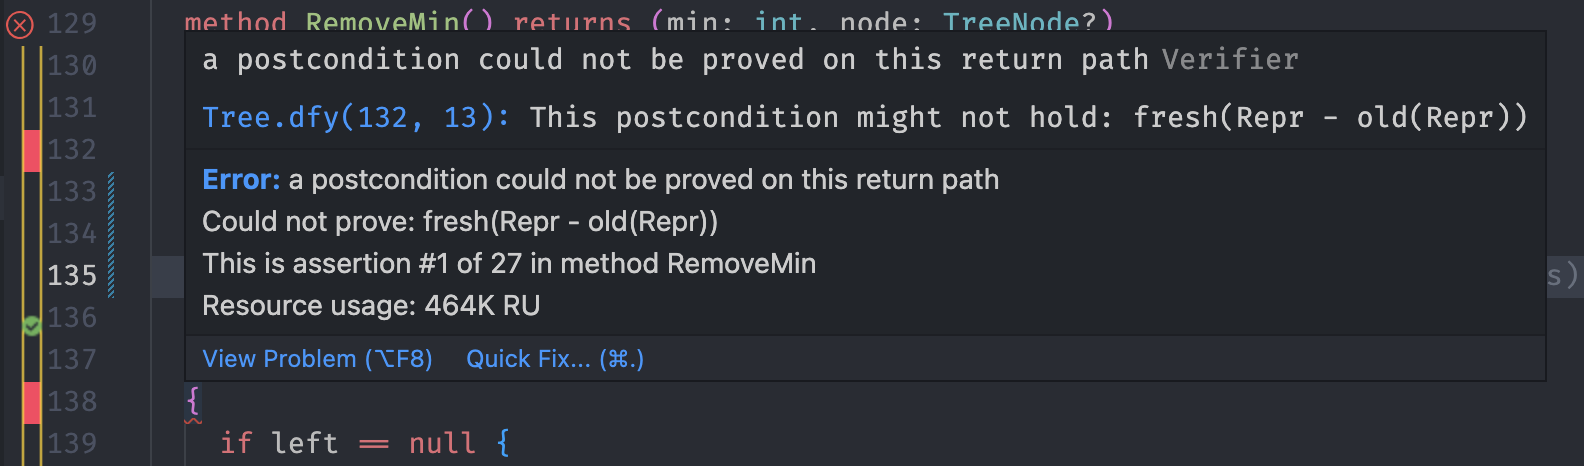
\includegraphics[scale=0.35]{./assets/images/error_example.png}
            \end{figure}
            \item La formalizzazione della specifica è resa possibile da \textit{keyword} riservate per le precondizioni, 
            postcondizioni, invarianti, metriche di terminazione e per il framing della 
            memoria nel caso in cui il programma abbia \textit{side effects}
        \end{itemize}    
    }
    \only<3>{
        \begin{itemize}
            \item Inoltre, per supportare ulteriormente la specifica, il linguaggio offre variabili \textit{ghost} aggiornabili,
            funzioni ricorsive e tipi come \textit{set} e liste
            \item I costrutti per la specifica e i costrutti \textit{ghost} vengono utilizzati unicamente durante la verifica
            e sono omessi dal programma eseguibile
            \item Il programma finale può essere compilato in altri linguaggi come ad esempio (C++, Java e Go) per permettere 
            l'integrazione in altri programmi
        \end{itemize}
    }
\end{frame}

\begin{frame}{Dafny: funzionamento}
    % Ora un veloce richiamo di teoria 
    % 1. Concetto alla base è quello di tripla di Hoare
    % 2. Per separare parte logica da parte sintattica usi wp calculus
    % 3. La formula che ottieni viene passata a SMT solver
    % 4. Grafico smt solver
    \only<1>{
    \begin{block}{Tripla di Hoare}
        \begin{center}
            \{P\}C\{Q\}     
        \end{center}
        Se l'asserzione \textit{P} è vera prima dell'esecuzione del comando \textit{C} allora l'asserzione \textit{Q} sarà vera al termine dell'esecuzione
    \end{block}
    \begin{block}{\textit{Predicate transformer semantics}}
        La semantica dei \textit{predicate transformer} è una riformulazione della logica di \textit{Floyd-Hoare} che definisce una strategia completa per la costruzione di deduzioni valide
    \end{block}
    \begin{block}{\textit{Weakest precondition}}
        Dato un comando \textit{C} e una postcondizione \textit{Q} la \textit{weakest precondition} (\textit{wp}) è un predicato \textit{$\phi$} tale per cui per ogni precondizione \textit{P}, \{P\}C\{Q\} se e solo se P$\implies \phi$
    \end{block}
    }
    \only<2>{
        \begin{figure}
            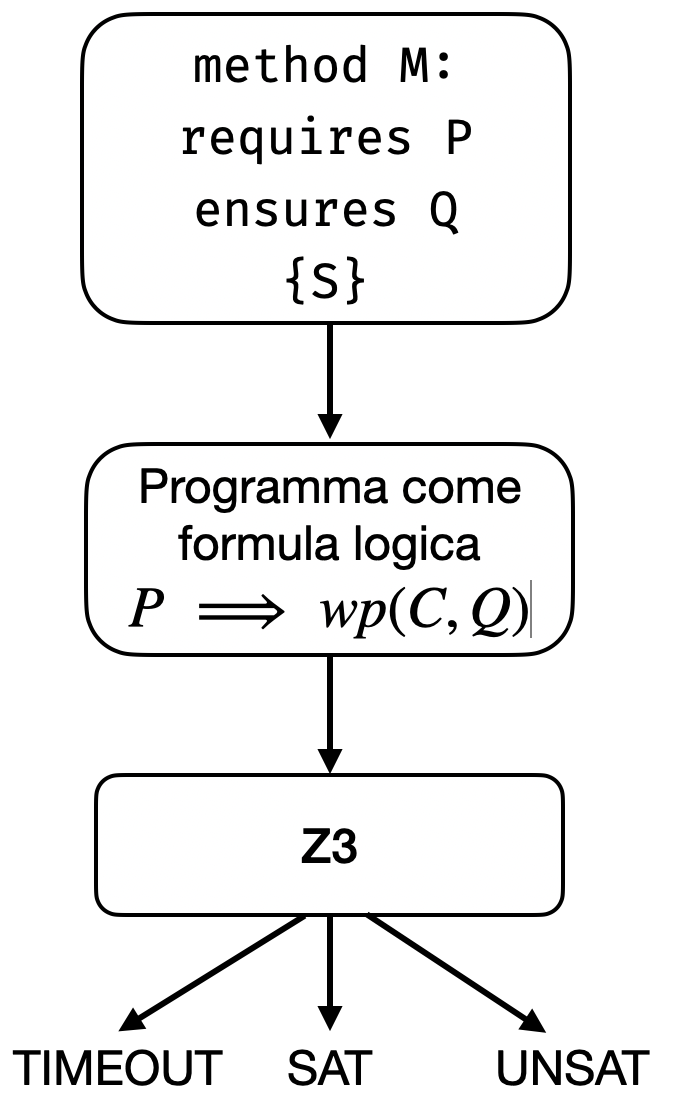
\includegraphics[scale=0.4]{./assets/images/mechanism.png}
        \end{figure}
    }
\end{frame}

\begin{frame}[containsverbatim]{Caratteristiche del linguaggio}
% Ora veramente in super sintesi le caratteristiche del linguaggio
% 1. Tipi
% 2. Generici
% 3. Predicati metodi e funzioni   
        \begin{itemize}
            \item I programmi Dafny sono principalmente composti da classi, metodi e predicati
            \begin{lstlisting}[basicstyle=\tiny]
class Nome {
    var nomeVar : tipo
    
    constructor(param : tipo)
        ensures _postcondizione_
    { Corpo.. }

    predicate Valid()
        reads _frame di memoria_
    { Corpo.. }

    method NomeMetodo (param : tipo) returns (valore : tipo)
        requires _precondizione_
        modifies _frame di memoria_
        ensures _postcondizione_
        decreases _metrica di terminazione_
    { Corpo.. }
}
            \end{lstlisting}
        \end{itemize}
\end{frame}

\begin{frame}{Caso di studio: BST}
% Albero binario di ricerca con veloce presentazione della struttura dati
    \begin{block}{Albero binario di ricerca}
        Un albero binario di ricerca è una struttura dati concatenata in cui ogni nodo è un oggetto.
        Ogni nodo al suo interno contiene una chiave e gli attributi \textit{left} e \textit{right} che puntano
        rispettivamente al figlio sinistro e al figlio destro
    \end{block}
    \begin{block}{Proprietà degli alberi binari di ricerca}
        Sia \textit{x} un nodo in un albero binario di ricerca. Se \textit{y} è un nodo nel sottoalbero sinistro
        di \textit{x} allora \textit{y.key} $< $ \textit{x.key}. Se \textit{y} è un nodo nel sottoalbero destro
        di \textit{x} allora \textit{y.key} $> $ \textit{x.key}
    \end{block}
\end{frame}

\begin{frame}{BST: variabili d'istanza}
    \lstinputlisting[]{./assets/code/bst_instance_var.dfy}
\end{frame}

\begin{frame}{BST: invariante di struttura}
    \lstinputlisting[basicstyle=\tiny]{./assets/code/bst_invariant.dfy}
\end{frame}

\begin{frame}{BST: costruttore}
    \lstinputlisting[]{./assets/code/bst_constructor.dfy}
\end{frame}

\begin{frame}{BST: inserimento}
    \lstinputlisting[basicstyle=\tiny]{./assets/code/bst_insert.dfy}
\end{frame}

\begin{frame}{BST: ricerca}
    \lstinputlisting[basicstyle=\tiny]{./assets/code/bst_find.dfy}
\end{frame}

\begin{frame}{BST: cancellazione}
    \only<1>{
        \lstinputlisting[basicstyle=\tiny]{./assets/code/bst_remove.dfy}
    }
    \only<2>{
        \lstinputlisting[basicstyle=\tiny]{./assets/code/bst_removeMin.dfy}
    }
\end{frame}

\end{document}
